\PassOptionsToPackage{quiet}{fontspec}
\documentclass[12pt,a4paper,UTF8]{article}
\usepackage{thesis} % 格式控制
\usepackage{amssymb} % 提供 \checkmark 等符号
\usepackage{indentfirst}
\usepackage{tikz}
\usepackage{tabularx}
\usetikzlibrary{arrows.meta}
\usetikzlibrary{positioning}
\setlength{\parindent}{2em} % 控制首行缩进  
\addtolength{\parskip}{3pt} % 控制段落距离  
\onehalfspacing % 1.5倍行距  
\graphicspath{{./figures/}} % 指定图片所在文件夹  


\classname{智能制造与企业自动化}  % 设置课程名称
\makepagestyle{}{\printclassname ~课程论文}




\begin{document}
\maketitlepage{面向交通扰动环境的TWVRP}{问题求解与鲁棒性分析}{教4 - 110}{董佳泽、白林颖、周茉}{\today}{赵均、徐祖华} %封面页 

\maketoc    %目录页
\section{绪论}
\label{sec:intro}
\subsection{研究背景}
车辆路径问题（Vehicle Routing Problem, VRP）是物流配送、生产调度与供应链管理中的经典组合优化问题，其核心目标是在给定客户需求、车辆资源和配送约束的条件下，规划一组车辆路线，使得所有客户能够被合理服务，并尽可能降低运输成本。对于制造企业而言，配送调度不仅涉及仓库到客户之间的运输过程，也可对应于厂区物料配送、零部件转运、成品出库配送等典型场景。因此，路径规划问题与制造企业自动化、智能物流和生产运营优化具有直接联系。

在基本 VRP 问题中，通常只考虑车辆容量和总运输距离等约束。然而在实际配送过程中，客户往往具有明确的服务时间要求。例如，企业客户可能只允许在指定工作时段收货，生产线工位也可能要求物料在特定时间段前送达。本文研究带容量约束的带时间窗车辆路径问题，即 Capacitated Vehicle Routing Problem with Time Windows。为行文简洁，后文统一记为 TWVRP。与普通 VRP 相比，TWVRP 不仅要求路径距离较短，还要求车辆到达客户的时间满足时间窗限制，因此路线规划不能简单按照空间距离最近原则进行，而需要综合考虑车辆当前时间、客户服务时间、等待时间和后续客户的可达性。

此外，在真实物流系统中，车辆行驶时间往往并非完全确定。道路拥堵、交通事故、天气变化和城市高峰期出行等因素都会导致实际行驶时间相对规划时间发生偏移。对于带时间窗约束的配送问题而言，行驶时间扰动会直接影响客户到达时刻，进而可能导致原本在静态条件下可行的路线在执行过程中出现时间窗违约。因此，仅研究确定性 TWVRP 仍然难以完整反映真实调度系统中的执行风险。基于此，本文在标准 TWVRP 求解的基础上，进一步引入交通扰动评估，用于分析静态规划路线在随机交通环境下的鲁棒性退化，并比较不同类型求解方法在解质量、运行效率和动态鲁棒性方面的差异。

\subsection{研究对象与任务目标}
本文研究对象为带时间窗容量约束车辆路径问题。给定一个配送中心、若干客户节点和一支容量受限的同质车队，每个客户具有需求量、服务时间和时间窗约束，求解器需要规划多条从配送中心出发并最终返回配送中心的车辆路线，使得每个客户被访问一次且仅一次，并在满足容量和时间窗约束的前提下尽可能降低总行驶成本。

本文采用 Solomon 与 Homberger 标准 TWVRP 数据集作为实验基准，覆盖 100、200、400、600、800 和 1000 客户规模。该类数据集包含客户坐标、需求量、时间窗、服务时间、车辆容量等信息，能够较好地用于验证不同求解算法在标准路径规划问题中的性能。围绕该问题，本文分别实现和分析三类求解器：基于 OR-Tools 的约束优化求解器、基于启发式规则与局部搜索的启发式求解器，以及基于神经组合优化和强化学习的学习型求解器。

本文的具体任务目标如下：

\begin{enumerate}
    \item 建立统一的 TWVRP 问题描述、数据读取流程和结果评价体系，使三类求解器能够在相同数据集和相同评价指标下进行比较。
    
    \item 实现基于 OR-Tools 的标准 TWVRP 求解器，将其作为确定性场景下的工业优化基线，分析其在不同规模实例上的可行性、成本和运行时间表现。
    
    \item 实现启发式算法求解器，通过规则构造初始解并结合局部搜索进行改进，分析其在求解速度、可解释性和解质量方面的特点。
    
    \item 实现基于强化学习的神经组合优化求解器，分析其在静态 TWVRP 求解中的快速推理能力，并进一步研究交通扰动下静态路线的退化现象和动态追索策略的改进效果。
    
    \item 在交通扰动评估下比较静态预规划、离线鲁棒预规划、在线启发式反应和强化学习动态追索等不同策略的性能差异，为制造企业物流调度中的算法选择提供参考。
\end{enumerate}
\subsection{研究方法与技术路线}
本文的整体研究路线可以概括为“统一建模、分别求解、统一评估、综合对比”。首先，根据 Solomon 与 Homberger 数据集中的客户坐标、需求量、时间窗和服务时间等字段，构建标准 TWVRP 实例，并统一车辆容量约束、时间窗约束和客户访问约束。随后，分别采用 OR-Tools、启发式算法和强化学习方法进行求解，得到车辆路径方案。最后，通过统一评估函数统计总行驶成本、车辆使用数、等待时间、时间窗违约率、容量违约率、可行率和运行时间等指标，并在交通扰动场景下进一步统计可行概率、平均 CVR 和极端情况下的违约风险。

在 OR-Tools 求解器部分，本文将 TWVRP 建模为约束优化问题。通过 Routing Model 表示多车辆路径，通过 Capacity Dimension 处理车辆容量约束，通过 Time Dimension 处理行驶时间、服务时间和客户时间窗约束，并结合初始解策略与局部搜索策略求解。OR-Tools 求解器的主要作用是提供确定性 TWVRP 场景下的高质量基线，并进一步用于分析静态最优或近优路线在交通扰动下的鲁棒性。

在启发式算法部分，本文采用规则驱动的构造方法和局部搜索改进方法。启发式算法不直接追求严格全局最优，而是通过较低计算成本快速生成可行或近似可行的路线方案，并通过 2-opt、relocate、swap 或禁忌搜索等邻域操作进行改进。该部分重点体现启发式方法实现简单、运行速度快和路径调整逻辑可解释等特点。

在强化学习求解器部分，本文将路径构造过程视为序列决策问题。静态规划器根据客户特征和当前车辆状态输出客户访问顺序，再由约束感知解码器构造满足容量和时间窗约束的多车辆路线。在交通扰动场景下，进一步采用静态引导的动态追索方法，即利用静态模型生成的基准路线构造动态训练数据，使在线决策网络在随机交通和时间窗变化条件下学习更稳健的调度策略。该方法的重点是分析学习型求解器在大规模实例上的快速推理能力和动态场景下的自适应能力。

本文技术路线如图~\ref{fig:intro_technical_route} 所示。

\begin{figure}[!htbp]
    \centering
    \begin{tikzpicture}[
        font=\small,
        node distance=1.0cm,
        block/.style={
            draw,
            rounded corners,
            align=center,
            minimum width=3.6cm,
            minimum height=0.9cm,
            inner sep=4pt
        },
        wideblock/.style={
            draw,
            rounded corners,
            align=center,
            minimum width=11.2cm,
            minimum height=0.9cm,
            inner sep=4pt
        },
        arrow/.style={-Latex, thick}
    ]
        \node[wideblock] (data) {Solomon / Homberger 数据集\\客户坐标、需求量、时间窗、服务时间、车辆容量};
        
        \node[wideblock, below=of data] (model) {标准 TWVRP 建模\\访问唯一性、容量约束、时间窗约束、车辆路径约束};
        
        \node[block, below left=1.1cm and -0.2cm of model] (ortools) {OR-Tools\\约束优化求解};
        \node[block, below=1.1cm of model] (heuristic) {启发式算法\\构造解 + 局部搜索};
        \node[block, below right=1.1cm and -0.2cm of model] (rl) {强化学习\\神经排序 + 动态追索};
        
        \node[wideblock, below=2.5cm of model] (eval) {统一评价指标\\总行驶成本、车辆数、等待时间、CVR、可行率、运行时间};
        
        \node[wideblock, below=of eval] (traffic) {交通扰动评估\\Monte Carlo 采样、可行概率、P95 CVR、迟到风险};
        
        \node[wideblock, below=of traffic] (compare) {三类求解器综合对比\\解质量、计算效率、可解释性、鲁棒性与适用场景};

        \draw[arrow] (data) -- (model);
        \draw[arrow] (model) -- (ortools);
        \draw[arrow] (model) -- (heuristic);
        \draw[arrow] (model) -- (rl);
        \draw[arrow] (ortools) |- (eval);
        \draw[arrow] (heuristic) -- (eval);
        \draw[arrow] (rl) |- (eval);
        \draw[arrow] (eval) -- (traffic);
        \draw[arrow] (traffic) -- (compare);
    \end{tikzpicture}
    \caption{技术路线}
    \label{fig:intro_technical_route}
\end{figure}
\subsection{主要工作}
围绕标准 TWVRP 求解与交通扰动下的鲁棒性分析，本文主要完成以下工作：

\begin{enumerate}
    \item \textbf{构建统一的 TWVRP 实验框架。}
    本文基于 Solomon 与 Homberger 标准数据集，统一整理客户坐标、需求量、时间窗、服务时间和车辆容量等输入信息，并建立统一的路径评估流程。为避免不同算法内部目标函数不一致造成比较偏差，本文在最终统计中统一使用外部评估函数计算总行驶成本、等待时间、时间窗违约、容量违约、可行率和运行时间等指标。

    \item \textbf{实现并分析 OR-Tools 确定性求解器。}
    本文采用 Google OR-Tools 对标准 TWVRP 进行建模求解，利用时间维度和容量维度分别处理时间窗约束和车辆容量约束。实验表明，OR-Tools 在确定性 TWVRP 场景下能够稳定获得高可行性路线，适合作为三类方法对比中的工业优化基线。进一步地，本文将 OR-Tools 静态路线置于比例交通扰动环境下进行 Monte Carlo 评估，用于分析静态最优路线在动态执行条件下的鲁棒性退化。

    \item \textbf{实现并分析启发式求解器。}
    本文设计基于启发式规则和局部搜索的 TWVRP 求解方法，通过构造初始路线、检查约束可行性并执行邻域改进，快速生成路径规划结果。该方法重点用于展示传统启发式算法在运行速度和可解释性方面的优势，并作为 OR-Tools 与强化学习方法之间的轻量级对照。
    
    \item \textbf{实现并分析强化学习求解器。}
    本文采用神经组合优化方法对 TWVRP 进行求解，通过神经网络生成客户访问顺序，并由约束感知解码器构造多车辆路线。在此基础上，进一步引入静态引导的动态追索方法，用静态规划路线构造交通扰动下的动态训练样本，使在线决策网络能够在随机交通场景中进行实时调整。该部分用于展示学习型方法在快速推理和动态鲁棒性方面的潜力。
    
    \item \textbf{完成三类求解器的综合对比分析。}
    本文从标准静态 TWVRP、交通扰动下的路线鲁棒性、运行时间随规模变化、成本与可行性权衡等角度对三类方法进行横向比较。通过对比分析，进一步总结 OR-Tools、启发式算法和强化学习方法在制造企业配送调度中的适用场景。
\end{enumerate}
\section{TWVRP 问题描述与数学建模}
\label{sec:twvrp_model}

\subsection{标准 TWVRP 问题描述}

带时间窗车辆路径问题（TWVRP）是在传统车辆路径问题基础上进一步引入客户服务时间约束的组合优化问题。给定一个配送中心、若干客户节点以及一支容量受限的车辆集合，求解器需要为车辆规划多条配送路线，使得每个客户被访问一次且仅一次，并在满足车辆容量约束和客户时间窗约束的前提下尽可能降低配送成本。

在本文研究的制造企业配送场景中，配送中心可以对应企业仓库、物流中心或生产物料集散点，客户节点可以对应外部客户、分销点或厂区内不同工位。每个客户具有一定的需求量，并要求车辆在给定时间窗内完成服务。车辆从配送中心出发，在服务若干客户后返回配送中心。由于车辆容量有限，同一辆车不能服务超过其载重能力的客户集合；由于客户具有时间窗约束，车辆即使在空间距离上能够较快到达，也可能由于到达过早而需要等待，或由于到达过晚而造成时间窗违约。

与普通 VRP 相比，TWVRP 的难点不只在于寻找空间距离较短的路径，还在于协调车辆到达时间与客户时间窗之间的关系。对于一条车辆路线而言，前序客户的服务时间、等待时间和行驶时间都会影响后续客户的到达时刻，因此局部最短路径选择不一定能够得到全局可行或高质量的配送方案。本文后续三类求解器均围绕该标准 TWVRP 问题展开，并在统一评估口径下比较其性能。

\subsection{符号定义}

设配送网络由节点集合 $V=\{0,1,\dots,n\}$ 构成，其中节点 $0$ 表示配送中心，客户集合记为 $N=\{1,2,\dots,n\}$。车辆集合记为 $K=\{1,2,\dots,m\}$，每辆车容量为 $Q$。客户 $i$ 的需求量为 $q_i$，服务时间为 $s_i$，时间窗为 $[e_i,l_i]$，其中 $e_i$ 表示最早允许服务时间，$l_i$ 表示最晚允许服务时间。节点 $i$ 到节点 $j$ 的行驶成本记为 $c_{ij}$，行驶时间记为 $t_{ij}$。在本文实验中，$c_{ij}$ 通常由距离矩阵或行驶时间矩阵给出。

主要符号定义如表~\ref{tab:twvrp_notation} 所示。

\begin{table}[!htbp]
    \centering
    \caption{TWVRP 主要符号定义}
    \label{tab:twvrp_notation}
    \small
    \begin{tabularx}{\textwidth}{p{3.0cm} X}
        \toprule
        符号 & 含义 \\
        \midrule
        $V$ & 所有节点集合，包含配送中心和客户节点 \\
        $N$ & 客户节点集合，$N=V\setminus\{0\}$ \\
        $K$ & 车辆集合 \\
        $0$ & 配送中心节点 \\
        $q_i$ & 客户 $i$ 的需求量 \\
        $Q$ & 单辆车最大容量 \\
        $[e_i,l_i]$ & 客户 $i$ 的服务时间窗 \\
        $s_i$ & 客户 $i$ 的服务时间 \\
        $c_{ij}$ & 节点 $i$ 到节点 $j$ 的行驶成本 \\
        $t_{ij}$ & 节点 $i$ 到节点 $j$ 的行驶时间 \\
        $x_{ijk}$ & 决策变量，若车辆 $k$ 从节点 $i$ 行驶到节点 $j$，则 $x_{ijk}=1$，否则为 $0$ \\
        $T_i$ & 客户 $i$ 的服务开始时间 \\
        $M$ & 足够大的常数，用于时间递推约束线性化 \\
        \bottomrule
    \end{tabularx}
\end{table}

\subsection{决策变量}

本文采用如下二进制决策变量描述车辆路径：

\[
x_{ijk}=
\begin{cases}
1, & \text{若车辆 } k \text{ 从节点 } i \text{ 行驶到节点 } j,\\
0, & \text{否则}.
\end{cases}
\]

同时，定义连续变量 $T_i$ 表示客户 $i$ 的服务开始时间。对于配送中心，可根据具体建模需要定义车辆出发时间和返回时间；在本文实验评估中，车辆默认从配送中心出发，并在完成其路线后返回配送中心。

\subsection{目标函数}

标准 TWVRP 的常见优化目标是最小化所有车辆的总行驶成本：

\begin{equation}
    \min \sum_{k\in K}\sum_{i\in V}\sum_{\substack{j\in V\\j\ne i}} c_{ij}x_{ijk}.
    \label{eq:twvrp_objective}
\end{equation}

其中，$c_{ij}$ 可以表示节点间欧氏距离、行驶时间或由实际道路网络得到的运输成本。本文在统一评价中将总行驶成本作为主要成本指标，同时将等待时间、车辆使用数、约束违约率和运行时间作为独立指标统计。这样可以避免不同求解器内部目标函数设置不同而导致结果不可比。

在部分求解器实现中，还可以在目标函数中加入车辆固定成本或等待时间惩罚项，以引导求解器减少车辆使用数或等待时间。但在最终对比分析中，本文统一采用外部评估函数重新计算指标，确保 OR-Tools、启发式算法和强化学习方法的结果具有一致的评价口径。

\subsection{约束条件}

\subsubsection{客户访问唯一性约束}

每个客户必须被访问一次且仅一次，即每个客户恰好有一条进入边：

\begin{equation}
    \sum_{k\in K}\sum_{\substack{i\in V\\i\ne j}}x_{ijk}=1,
    \quad \forall j\in N.
    \label{eq:visit_once_in}
\end{equation}

同时，每个客户也恰好有一条离开边：

\begin{equation}
    \sum_{k\in K}\sum_{\substack{j\in V\\j\ne i}}x_{ijk}=1,
    \quad \forall i\in N.
    \label{eq:visit_once_out}
\end{equation}

该约束保证所有客户均被服务，且不存在客户遗漏或重复访问。

\subsubsection{车辆出发与返回约束}

每辆被使用的车辆从配送中心出发，并最终返回配送中心。对于车辆 $k$，其从配送中心出发的次数与返回配送中心的次数应相等：

\begin{equation}
    \sum_{j\in N}x_{0jk}
    =
    \sum_{i\in N}x_{i0k},
    \quad \forall k\in K.
    \label{eq:depot_balance}
\end{equation}

若每辆车最多使用一次，则有：

\begin{equation}
    \sum_{j\in N}x_{0jk}\leq 1,
    \quad \forall k\in K.
    \label{eq:vehicle_use_once}
\end{equation}

该约束确保每条路线均以配送中心为起点和终点。

\subsubsection{流守恒约束}

对于任一客户节点，如果某辆车进入该客户节点，则该车辆也必须从该客户节点离开：

\begin{equation}
    \sum_{\substack{i\in V\\i\ne h}}x_{ihk}
    =
    \sum_{\substack{j\in V\\j\ne h}}x_{hjk},
    \quad \forall h\in N,\ \forall k\in K.
    \label{eq:flow_conservation}
\end{equation}

流守恒约束保证车辆路线在客户节点处连续，不会出现车辆进入后不离开或无前序节点直接离开的情况。

\subsubsection{容量约束}

每辆车服务的客户总需求量不能超过车辆容量：

\begin{equation}
    \sum_{i\in N}q_i
    \left(
        \sum_{\substack{j\in V\\j\ne i}}x_{ijk}
    \right)
    \leq Q,
    \quad \forall k\in K.
    \label{eq:capacity_constraint}
\end{equation}

该约束反映了车辆装载能力限制，是容量约束车辆路径问题的基本约束之一。

\subsubsection{时间递推约束}

若车辆从客户 $i$ 行驶到客户 $j$，则客户 $j$ 的服务开始时间必须不早于客户 $i$ 的服务完成时间加上从 $i$ 到 $j$ 的行驶时间。该关系可表示为：

\begin{equation}
    T_j
    \geq
    T_i+s_i+t_{ij}
    -M(1-x_{ijk}),
    \quad \forall i,j\in N,\ i\ne j,\ \forall k\in K.
    \label{eq:time_propagation}
\end{equation}

其中，$M$ 为足够大的常数。当 $x_{ijk}=1$ 时，式~\eqref{eq:time_propagation} 约束车辆访问顺序下的时间递推关系；当 $x_{ijk}=0$ 时，该约束被放松。

对于从配送中心出发到第一个客户，或从最后一个客户返回配送中心的情况，也可以采用类似形式进行时间递推。本文在算法实现中通过时间维度或路径仿真过程统一维护车辆当前时间。

\subsubsection{时间窗约束}

每个客户的服务开始时间必须位于其时间窗内：

\begin{equation}
    e_i \leq T_i \leq l_i,
    \quad \forall i\in N.
    \label{eq:time_window_constraint}
\end{equation}

若车辆早于 $e_i$ 到达客户 $i$，则允许车辆等待，直到 $e_i$ 后开始服务；若车辆晚于 $l_i$ 到达，则该客户发生时间窗违约。标准 TWVRP 通常将时间窗作为硬约束，即不允许任何时间窗违约。本文在标准静态求解中采用硬时间窗约束，在交通扰动评估中则统计扰动执行后的时间窗违约情况，用于分析静态路线的鲁棒性。

\subsubsection{决策变量约束}

路径决策变量为二进制变量：

\begin{equation}
    x_{ijk}\in\{0,1\},
    \quad \forall i,j\in V,\ i\ne j,\ \forall k\in K.
    \label{eq:binary_constraint}
\end{equation}

服务开始时间变量为非负连续变量：

\begin{equation}
    T_i\geq 0,
    \quad \forall i\in V.
    \label{eq:time_nonnegative}
\end{equation}

\subsection{路线执行过程与等待时间计算}

对于任意一条车辆路线
\[
r=(0,i_1,i_2,\dots,i_p,0),
\]
其执行过程可通过车辆当前时间逐步递推。设车辆从配送中心出发时刻为 $0$，到达客户 $i_h$ 的时刻为 $A_{i_h}$，服务开始时刻为 $T_{i_h}$，则有：

\begin{equation}
    A_{i_h}=T_{i_{h-1}}+s_{i_{h-1}}+t_{i_{h-1},i_h},
    \quad h=1,2,\dots,p.
    \label{eq:arrival_time}
\end{equation}

若车辆提前到达客户，则需要等待：

\begin{equation}
    W_{i_h}=\max(0,e_{i_h}-A_{i_h}).
    \label{eq:waiting_time}
\end{equation}

客户实际服务开始时间为：

\begin{equation}
    T_{i_h}=\max(A_{i_h},e_{i_h}).
    \label{eq:service_start_time}
\end{equation}

若 $T_{i_h}>l_{i_h}$，则客户 $i_h$ 发生时间窗违约。由此可见，等待时间虽然不一定直接计入总行驶成本，但会影响后续客户的服务开始时间，是 TWVRP 评估中的重要指标。

\subsection{交通扰动评估模型}

标准 TWVRP 假设节点间行驶时间 $t_{ij}$ 是确定的。然而在实际配送过程中，交通状态具有随机性。为了评估静态规划路线在动态交通环境下的执行风险，本文进一步引入比例交通扰动模型，对规划得到的路线进行 Monte Carlo 仿真评估。

设 $T^{base}_{ij}$ 为节点 $i$ 到节点 $j$ 的基准行驶时间，$d_{ij}$ 为两节点间的欧氏距离，则扰动后的行驶时间定义为：

\begin{equation}
    T^{perturbed}_{ij}
    =
    \max\left(
        T_{\min},
        T^{base}_{ij}
        \left[
            1+
            \lambda\sigma_{traffic}\varepsilon
            \left(1-e^{-d_{ij}/50}\right)
        \right]
    \right),
    \quad
    \varepsilon \sim \mathcal{N}(0,1).
    \label{eq:traffic_perturbation}
\end{equation}

其中，$\sigma_{traffic}$ 表示交通扰动标准强度，$\lambda$ 表示扰动强度倍数，$\varepsilon$ 为服从标准正态分布的随机变量，$\left(1-e^{-d_{ij}/50}\right)$ 为距离相关放大项。该项表示长距离边更容易受到交通不确定性的影响，而短距离边受到的扰动相对较小。为避免扰动后行驶时间出现不合理取值，实际仿真中设置如下下界：

\begin{equation}
    T_{\min}=\max(1,0.1T^{base}_{ij}).
    \label{eq:traffic_lower_bound}
\end{equation}

在交通扰动评估中，给定一组已规划路线，本文对每个实例重复采样多次随机交通实现，并重新模拟车辆沿原路线执行的过程。对于每次仿真，统计其总行驶成本、时间窗违约数、容量违约数和迟到时间等指标。最终通过多次采样的均值、标准差和分位数刻画路线在随机交通环境下的鲁棒性。

\subsection{评价指标定义}
为统一比较 OR-Tools、启发式算法和强化学习方法，本文采用外部评估函数对各求解器输出路线进行统一评价。具体指标定义、统计口径和交通扰动下的鲁棒性指标见第~\ref{sec:dataset_eval}~节，本节不再重复展开。

\subsection{问题设置}

综上，本文主要研究两个层次的问题。第一层是标准确定性 TWVRP 求解，即在给定确定性行驶时间矩阵的条件下，分别使用 OR-Tools、启发式算法和强化学习方法构造满足容量和时间窗约束的车辆路线，并比较其成本、可行性和运行时间。第二层是在静态路线基础上引入交通扰动评估，分析确定性预规划路线在随机交通环境下的鲁棒性变化，并进一步比较离线鲁棒预规划和强化学习动态追索等策略的表现。

通过上述建模方式，本文将三类求解器统一到相同问题定义和相同评价体系下，从而为后续章节的算法设计与实验对比奠定基础。



\section{数据集与实验评价体系}
\label{sec:dataset_eval}

\subsection{数据集结构}

本文采用 Solomon 与 Homberger 标准 TWVRP 数据集作为实验基准。Solomon 数据集主要用于 100 客户规模的 VRPTW 测试，Homberger 数据集在 Solomon 数据集基础上扩展到 200、400、600、800 和 1000 客户规模，适合用于检验算法在大规模带时间窗车辆路径问题中的扩展能力。

每个 TWVRP 实例由一个配送中心、若干客户节点和一组车辆资源构成。配送中心作为所有车辆的出发点和返回点，客户节点包含空间位置、需求量、服务时间和时间窗等信息。车辆具有固定容量，求解器需要在容量和时间窗约束下规划多条车辆路线，使每个客户被访问一次且仅一次。

数据集中主要字段如表~\ref{tab:dataset_structure} 所示。

\begin{table}[!htbp]
    \centering
    \caption{TWVRP 数据集主要字段}
    \label{tab:dataset_structure}
    \small
    \begin{tabularx}{\textwidth}{p{3.2cm} p{4.0cm} X}
        \toprule
        字段 & 含义 & 作用 \\
        \midrule
        Customer ID & 客户编号 & 用于区分不同客户节点，并构造车辆访问序列 \\
        Coordinates & 节点二维坐标 & 用于计算节点间距离或行驶时间矩阵 \\
        Demand & 客户需求量 & 用于判断车辆路线是否满足容量约束 \\
        Ready Time & 最早服务时间 & 客户时间窗下界，车辆早到时需要等待 \\
        Due Time & 最晚服务时间 & 客户时间窗上界，车辆晚到时产生时间窗违约 \\
        Service Time & 服务时间 & 表示车辆在客户处完成服务所需时间，影响后续到达时间 \\
        Vehicle Capacity & 车辆容量 & 限制单辆车可服务客户的总需求量 \\
        Number of Vehicles & 可用车辆数 & 限制最多可使用的车辆路线数量 \\
        \bottomrule
    \end{tabularx}
\end{table}

本文实验覆盖的主要规模如表~\ref{tab:dataset_scale_simple} 所示。不同规模实例用于评估 OR-Tools、启发式算法和强化学习求解器在小规模、中等规模和大规模 TWVRP 问题上的性能变化。

\begin{table}[!htbp]
    \centering
    \caption{实验数据规模}
    \label{tab:dataset_scale_simple}
    \small
    \begin{tabularx}{\textwidth}{p{2.5cm} p{2.8cm} p{2.8cm} X}
        \toprule
        规模 & 客户数 & 车辆容量 & 说明 \\
        \midrule
        100 & 100 & 200 & Solomon 标准规模，用于基础求解能力验证 \\
        200 & 200 & 200 & Homberger 扩展规模，用于中等规模测试 \\
        400 & 400 & 200 & 中大规模实例，用于分析算法扩展性 \\
        600 & 600 & 200 & 大规模实例，路线数量和时间窗约束明显增加 \\
        800 & 800 & 200 & 大规模实例，用于检验求解稳定性 \\
        1000 & 1000 & 200 & 最大测试规模，用于分析算法极限表现 \\
        \bottomrule
    \end{tabularx}
\end{table}

在数据预处理阶段，本文将配送中心统一编号为 $0$，客户节点编号为 $1$ 至 $n$。若数据文件中未直接给出行驶时间矩阵，则根据客户坐标计算欧氏距离：

\begin{equation}
    d_{ij}
    =
    \sqrt{(x_i-x_j)^2+(y_i-y_j)^2}.
    \label{eq:dataset_distance_simple}
\end{equation}

其中，$(x_i,y_i)$ 和 $(x_j,y_j)$ 分别为节点 $i$ 和节点 $j$ 的二维坐标。距离矩阵或时间矩阵作为三类求解器的共同输入，用于计算路径成本、车辆到达时间和时间窗可行性。

\subsection{评价指标}

由于 OR-Tools、启发式算法和强化学习方法的内部优化目标并不完全一致，本文不直接比较各求解器内部返回的目标函数值，而是将其输出路线输入统一评估函数，按照相同口径重新计算评价指标。

本文最终使用的主要评价指标如表~\ref{tab:final_metrics} 所示。

\begin{table}[!htbp]
    \centering
    \caption{最终性能评价指标}
    \label{tab:final_metrics}
    \small
    \begin{tabularx}{\textwidth}{p{3.5cm} p{4.4cm} X}
        \toprule
        指标 & 含义 & 评价作用 \\
        \midrule
        Total Cost & 所有车辆路线的总行驶成本 & 衡量路径解质量，数值越低表示路线越短或行驶代价越小 \\
        Per-customer Cost & 总行驶成本除以客户数量 & 消除规模差异后比较单位客户配送成本 \\
        Vehicles Used & 实际使用车辆数量 & 衡量车辆资源消耗情况 \\
        Waiting Time/min & 车辆早到客户后产生的累计等待时间 & 衡量路线与客户时间窗的匹配程度 \\
        CVR & 约束违约率 & 综合衡量时间窗和容量约束违反程度 \\
        Feasibility Rate & 可行率 & 衡量算法在测试实例中获得完全可行解的比例 \\
        Runtime/s & 求解或推理时间 & 衡量算法计算效率 \\
        Feasible Probability & 交通扰动仿真下的可行概率 & 衡量静态路线在随机交通环境下的鲁棒性 \\
        P95 CVR & 多次交通扰动仿真中 CVR 的 95\% 分位数 & 衡量极端交通情形下的尾部违约风险 \\
        \bottomrule
    \end{tabularx}
\end{table}

其中，总行驶成本定义为所有车辆路线中相邻节点行驶成本之和：

\begin{equation}
    C_{travel}
    =
    \sum_{r\in R}
    \sum_{h=0}^{|r|-2}
    c_{r_h,r_{h+1}},
    \label{eq:metric_total_cost}
\end{equation}

式中，$R$ 表示所有车辆路线集合，$r_h$ 表示路线 $r$ 中第 $h$ 个节点，$c_{r_h,r_{h+1}}$ 表示相邻节点之间的行驶成本。本文将行驶成本与等待时间分开统计，避免将运输代价和时间窗等待混合。

约束违约率（Constraint Violation Rate, CVR）定义为：

\begin{equation}
    CVR
    =
    100
    \cdot
    \frac{
        N_{tw}^{vio}+N_{cap}^{vio}
    }{
        N_{cust}
    },
    \label{eq:metric_cvr_simple}
\end{equation}

其中，$N_{tw}^{vio}$ 表示时间窗违约数量，$N_{cap}^{vio}$ 表示容量违约数量，$N_{cust}$ 表示客户总数。当 $CVR=0$ 且不存在客户遗漏或重复访问时，该路线被认为在确定性场景下完全可行。

在交通扰动评估中，同一条静态路线会在多个随机交通实现下重复仿真。可行概率定义为：

\begin{equation}
    P_{feas}
    =
    \frac{N_{feas}}{N_{MC}},
    \label{eq:metric_feasible_probability_simple}
\end{equation}

其中，$N_{MC}$ 表示 Monte Carlo 交通扰动采样次数，$N_{feas}$ 表示其中完全满足访问、容量和时间窗约束的仿真次数。$P_{feas}$ 越高，说明该路线在随机交通环境下越稳定。

为了描述极端交通条件下的风险，本文进一步统计 $P95$ CVR：

\begin{equation}
    CVR_{95}
    =
    \mathrm{Percentile}_{95}
    \left(
        CVR^{(1)},CVR^{(2)},\dots,CVR^{(N_{MC})}
    \right),
    \label{eq:metric_p95_cvr_simple}
\end{equation}

其中，$CVR^{(r)}$ 表示第 $r$ 次交通扰动仿真中的约束违约率。相比平均 CVR，$P95$ CVR 更能反映较差交通条件下的时间窗违约风险。

综上，本文采用统一的评价指标对三类求解器进行比较。在确定性 TWVRP 场景下，重点关注总行驶成本、车辆使用数、CVR、可行率和运行时间；在交通扰动场景下，进一步关注可行概率和 $P95$ CVR，以分析静态路线和动态追索策略的鲁棒性。


\clearpage
\section{启发式求解器设计}
\label{sec:heuristic}

\subsection{求解器总体建模与评价框架}

\subsubsection{启发式求解总体流程}

\subsection{启发式算法设计}
\subsubsection{NN+2-opt初始求解器}

\subsubsection{基础禁忌搜索算法}

\subsubsection{融合2-opt*的改进禁忌搜索}

\subsection{静态模式}


\subsection{混合约束模式}

\subsection{交通扰动模式}

\clearpage
\section{OR-Tools 求解器设计}
\label{sec:ortools}

前文已经对 TWVRP 的问题定义、数学模型、数据集结构和评价指标进行了说明。本节进一步介绍基于 OR-Tools 的 TWVRP 求解器设计方法。OR-Tools 是 Google 开源的组合优化工具包，其中 Routing Library 能够对车辆路径问题、带时间窗车辆路径问题和容量约束车辆路径问题进行建模求解。与启发式算法和强化学习方法相比，OR-Tools 的优势在于约束建模清晰、工程实现成熟、可行性保障能力较强，适合作为本文标准 TWVRP 问题的确定性优化基线。

在本文中，OR-Tools 求解器并不只用于给出一组静态路径结果，还承担两方面作用：一方面，在确定性行驶时间矩阵下求解标准 TWVRP，用于验证在硬时间窗和容量约束下能否稳定获得高质量可行解；另一方面，将其输出的静态路线置于交通扰动环境下进行仿真评估，用于分析传统离线预规划方法在随机交通场景中的鲁棒性边界。因此，本节的重点不是单纯介绍 OR-Tools 的基本用法，而是说明如何将第~\ref{sec:twvrp_model}~节中的 TWVRP 数学模型映射到 OR-Tools 的 RoutingModel、Time Dimension 和 Capacity Dimension 中，并进一步结合统一评价函数对输出路线进行评估。

\subsection{求解器设计目标}

OR-Tools 求解器的首要目标是在标准确定性 TWVRP 场景下构造满足约束的车辆路线。具体而言，给定客户坐标、需求量、时间窗、服务时间、车辆容量和可用车辆数，求解器需要输出若干条从配送中心出发并最终返回配送中心的车辆路线，使得所有客户被访问一次且仅一次，同时满足车辆容量约束和客户时间窗约束。在满足可行性的基础上，求解器进一步优化车辆使用数和总行驶成本，从而为本文三类求解器的横向比较提供可解释的工业优化基线。

与第~\ref{sec:twvrp_model}~节中的数学模型相对应，OR-Tools 求解器需要实现以下约束和目标：

\begin{enumerate}
    \item \textbf{客户访问约束：}每个客户节点必须被某一辆车访问一次，且不能出现遗漏客户或重复访问客户。
    
    \item \textbf{车辆路径约束：}每条车辆路线均从配送中心出发，并在完成客户服务后返回配送中心。
    
    \item \textbf{容量约束：}每辆车所服务客户的总需求量不能超过车辆容量。
    
    \item \textbf{时间窗约束：}车辆到达客户后，若早于客户最早服务时间，则允许等待；若晚于客户最晚服务时间，则该路线在标准硬时间窗问题中不可行。
    
    \item \textbf{服务时间约束：}车辆在客户处完成服务需要消耗对应服务时间，服务时间会影响后续客户的到达时刻，但不直接作为最终行驶成本统计。
    
    \item \textbf{优化目标：}在满足上述约束的基础上，尽可能减少车辆使用数和总行驶成本。
\end{enumerate}

本文将 OR-Tools 求解器定位为三类求解方法中的确定性优化基线，其设计目标如表~\ref{tab:ortools_design_goal} 所示。

\begin{table}[!htbp]
    \centering
    \caption{OR-Tools 求解器在本文中的设计目标}
    \label{tab:ortools_design_goal}
    \small
    \begin{tabularx}{\textwidth}{p{3.2cm} p{4.2cm} X}
        \toprule
        目标类别 & 具体目标 & 说明 \\
        \midrule
        确定性求解基线 &
        在标准 TWVRP 实例上获得高可行性路线 &
        用于验证 OR-Tools 在硬时间窗和容量约束下的基础求解能力，并作为三类算法横向对比的参考基线 \\
        \midrule
        约束建模验证 &
        显式处理客户访问、容量、时间窗和服务时间约束 &
        通过 RoutingModel、Capacity Dimension 和 Time Dimension 将数学模型转化为可求解的工程模型 \\
        \midrule
        解质量评估 &
        在满足可行性的前提下降低总行驶成本和车辆使用数 &
        反映传统优化求解器在确定性离线调度中的成本优化能力 \\
        \midrule
        交通扰动分析 &
        将静态路线放入随机交通环境下进行仿真 &
        用于分析确定性可行路线在动态执行条件下是否仍能保持可行 \\
        \midrule
        鲁棒预规划对照 &
        构造 mean、P90 和 mean+std 等保守规划矩阵 &
        用于说明传统离线优化方法在交通不确定性下的改进方式及其成本代价 \\
        \bottomrule
    \end{tabularx}
\end{table}

\subsection{OR-Tools 建模流程}

本文基于 Google OR-Tools Routing Solver 构建标准 TWVRP 求解器。与直接编写整数规划模型不同，OR-Tools Routing Solver 将车辆路径问题抽象为节点索引、车辆索引、路径弧成本和若干维度约束的组合优化模型。对于本文研究的 TWVRP 问题，求解器需要同时处理客户访问顺序、车辆容量、客户时间窗、服务时间和车辆数量等因素。因此，本文将第~\ref{sec:twvrp_model}~节中的数学模型映射为 OR-Tools 中的 \texttt{RoutingIndexManager}、\texttt{RoutingModel}、弧成本回调函数、时间维度和容量维度。

本文最终采用的 OR-Tools 建模流程如图~\ref{fig:ortools_modeling_flow} 所示。首先，读取 TWVRP 实例中的节点坐标、需求量、时间窗、服务时间、车辆容量和车辆数量等信息，并生成或读取节点间行驶时间矩阵。随后，使用 \texttt{RoutingIndexManager} 建立原始节点编号与 OR-Tools 内部索引之间的映射关系，再使用 \texttt{RoutingModel} 构造多车辆路径优化模型。在模型中，弧成本回调函数用于描述节点间行驶成本，时间维度用于描述车辆时间递推、等待时间和客户时间窗约束，容量维度用于描述车辆载重约束。求解完成后，模型输出每辆车的客户访问序列，并通过统一评价函数重新计算总行驶成本、等待时间、CVR 和可行性等指标。

\begin{figure}[!htbp]
    \centering
    \includegraphics[width=1\linewidth]{OR-Tools建模流程.png}
    \caption{OR-Tools 求解器建模流程}
    \label{fig:ortools_modeling_flow}
\end{figure}

\subsubsection{实例数据准备}

对于每个 TWVRP 实例，求解器首先整理 OR-Tools 建模所需的基础数据。节点数量记为 $n$，车辆数量记为 $m$，配送中心固定为节点 $0$。客户需求、服务时间、时间窗和车辆容量分别整理为数组形式：

\[
    \mathbf{q}=(q_0,q_1,\dots,q_n),
    \quad
    \mathbf{s}=(s_0,s_1,\dots,s_n),
    \quad
    \mathbf{tw}_i=[e_i,l_i],
    \quad
    \mathbf{Q}=(Q_1,Q_2,\dots,Q_m).
\]

由于 OR-Tools Routing Solver 的回调函数需要返回整数值，本文在建模阶段将行驶时间、服务时间和时间窗边界统一转换为整数分钟，从而保证模型内部时间递推的一致性。

\subsubsection{索引管理与路径模型构造}

OR-Tools 内部并不直接使用原始客户编号，而是通过 \texttt{RoutingIndexManager} 维护原始节点编号、车辆编号和路径变量索引之间的映射关系。本文采用单仓库设置，所有车辆均从节点 $0$ 出发并最终返回节点 $0$，因此索引管理器可表示为：

\[
    \texttt{RoutingIndexManager}(n, m, 0).
\]

在建立索引管理器后，进一步构造 \texttt{RoutingModel}，用于描述多辆车在客户节点之间的访问路径。该模型自动维护路径连续性和车辆起终点结构，因此第~\ref{sec:twvrp_model}~节中的客户访问约束、车辆出发返回约束和流守恒约束，在 OR-Tools 中主要由 \texttt{RoutingModel} 的路径结构实现。

\subsubsection{弧成本回调函数}

本文采用独立的弧成本回调函数描述节点间行驶成本。对于 OR-Tools 内部给定的 \texttt{from\_index} 和 \texttt{to\_index}，首先通过索引管理器将其转换为原始节点编号 $i$ 和 $j$，然后返回行驶时间矩阵中的 $t_{ij}$：

\[
    cost(i,j)=t_{ij}.
\]

该回调函数通过 \texttt{SetArcCostEvaluatorOfAllVehicles} 作用于所有车辆，用于引导 OR-Tools 最小化车辆路线的总行驶成本。需要注意的是，本文将弧成本回调与时间维度回调分开设置：弧成本只统计节点间行驶成本，不包含客户服务时间。这样可以保证最终优化目标与第~\ref{sec:dataset_eval}~节中定义的 Total Cost 口径一致，即总成本主要反映车辆行驶代价，而服务时间只影响路线的时间可行性。

\subsubsection{时间维度建模}

TWVRP 与普通 CVRP 的主要差异在于客户具有时间窗约束。本文通过 OR-Tools 的 \texttt{Time Dimension} 建模车辆时间递推、等待时间和客户时间窗。时间维度的 transit callback 定义为：

\[
    time(i,j)=t_{ij}+s_i,
\]

其中，$t_{ij}$ 为车辆从节点 $i$ 到节点 $j$ 的行驶时间，$s_i$ 为车辆在节点 $i$ 的服务时间。该定义表示车辆从节点 $i$ 出发前需要先完成节点 $i$ 的服务，再行驶至节点 $j$。因此，时间维度中的累计变量可以理解为车辆在路径执行过程中的时间状态。

在添加时间维度时，本文允许车辆在客户处等待。若车辆早于客户时间窗下界 $e_i$ 到达，则可以通过时间维度中的 slack 变量等待至 $e_i$ 后开始服务；若车辆晚于客户时间窗上界 $l_i$，则该路线违反硬时间窗约束。对于每个客户节点 $i$，本文通过如下方式设置硬时间窗：

\[
    C_i \in [e_i,l_i],
\]

其中，$C_i$ 表示 OR-Tools 时间维度中客户节点 $i$ 对应的累计时间变量。在实现中，该约束由 \texttt{CumulVar(index).SetRange($e_i,l_i$)} 完成。对于配送中心起点，本文将每辆车的起始时间固定为 $0$；对于车辆终点，则要求其返回时间不超过配送中心允许的最大时间范围。

\subsubsection{容量维度建模}

车辆容量约束通过 OR-Tools 的 \texttt{Capacity Dimension} 实现。本文定义需求回调函数，当车辆访问节点 $i$ 时返回该节点需求量 $q_i$，其中配送中心需求为 $0$。随后使用 \texttt{AddDimensionWithVehicleCapacity} 为每辆车设置最大容量 $Q_k$，使得任意车辆路径上累计客户需求不超过车辆容量：

\[
    \sum_{i\in r_k} q_i \leq Q_k,
    \quad \forall k\in K.
\]

其中，$r_k$ 表示车辆 $k$ 的访问客户集合。容量维度的累计变量会随着车辆访问客户而增加，若某条路径的累计需求超过车辆容量，则该路径在模型中不可行。

\subsubsection{车辆数量控制与目标引导}

Solomon/Homberger TWVRP 通常同时关注车辆数量和行驶距离。本文在 OR-Tools 模型中通过 \texttt{SetFixedCostOfAllVehicles} 为每辆被使用车辆设置固定成本，使求解器优先减少车辆使用数，并在车辆数量相同或相近的情况下进一步优化总行驶成本。其目标引导可以理解为：

\[
    \min \left(
        M_v \cdot N_{vehicle}
        +
        \sum_{k\in K}\sum_{(i,j)\in r_k} t_{ij}
    \right),
\]

其中，$M_v$ 为车辆固定成本系数，$N_{vehicle}$ 为实际使用车辆数。由于 $M_v$ 设置为较大的常数，减少一辆车通常比局部缩短路线距离具有更高优先级，从而符合标准 TWVRP 中先减少车辆数、再降低行驶距离的优化习惯。

\subsubsection{搜索参数与路线提取}

模型构建完成后，本文采用 OR-Tools 的启发式搜索流程进行求解。最终实验中，初始解策略采用 \texttt{PARALLEL\_CHEAPEST\_INSERTION}，用于快速构造满足约束的初始路径；局部搜索元启发式采用 \texttt{GUIDED\_LOCAL\_SEARCH}，用于在初始解基础上进一步降低目标函数值。求解时间由实验参数统一控制，以便在不同规模实例上比较运行效率。

求解完成后，本文从 OR-Tools 解对象中逐辆车提取访问序列。对于车辆 $k$，从其起点索引开始，按照 \texttt{NextVar} 变量依次读取后继节点，直到到达终点索引为止，从而得到形如

\[
    r_k=(0,i_1,i_2,\dots,i_p,0)
\]

的车辆路线。若某辆车未服务任何客户，则该车辆不计入实际使用车辆数。最终，所有非空车辆路线组成求解器输出结果，并输入统一评价函数进行后处理统计。

\begin{table}[!htbp]
    \centering
    \caption{TWVRP 约束与 OR-Tools 建模组件的对应关系}
    \label{tab:ortools_model_mapping}
    \small
    \begin{tabularx}{\textwidth}{p{3.8cm} p{4.2cm} X}
        \toprule
        TWVRP 建模内容 & OR-Tools 实现组件 & 说明 \\
        \midrule
        客户访问与路径连续性 &
        \texttt{RoutingModel} &
        通过路径变量和车辆起终点结构维护客户访问顺序与车辆路线连续性 \\
        \midrule
        节点编号与车辆编号映射 &
        \texttt{RoutingIndexManager} &
        建立原始节点编号、车辆编号和 OR-Tools 内部索引之间的映射 \\
        \midrule
        总行驶成本 &
        Arc Cost Callback &
        返回节点间行驶时间 $t_{ij}$，作为路径弧成本 \\
        \midrule
        服务时间与时间递推 &
        Time Transit Callback &
        返回 $t_{ij}+s_i$，将客户服务时间嵌入时间维度 \\
        \midrule
        客户时间窗 &
        \texttt{Time Dimension} 与 \texttt{CumulVar.SetRange} &
        对每个客户节点设置累计时间变量上下界 $[e_i,l_i]$ \\
        \midrule
        早到等待 &
        Time Dimension Slack &
        允许车辆早到后等待至客户时间窗开始 \\
        \midrule
        车辆容量约束 &
        \texttt{Capacity Dimension} &
        根据客户需求量累计车辆载重，并限制不超过车辆容量 \\
        \midrule
        车辆数量控制 &
        \texttt{SetFixedCostOfAllVehicles} &
        为每辆被使用车辆设置固定成本，引导求解器减少车辆数 \\
        \bottomrule
    \end{tabularx}
\end{table}

通过上述建模流程，本文将 TWVRP 中的客户访问、车辆容量、服务时间和时间窗约束统一转化为 OR-Tools Routing Solver 中的路径结构和维度约束。该方式既保留了 TWVRP 数学模型的主要约束，也便于在求解完成后将路线输出到统一评估模块中，从而与启发式算法和强化学习求解器进行同口径比较。

\subsection{交通扰动评估与鲁棒预规划}

前述 OR-Tools 建模流程主要面向确定性 TWVRP，即在给定固定行驶时间矩阵的条件下规划满足容量和时间窗约束的车辆路线。然而，在实际配送过程中，车辆行驶时间会受到道路拥堵、随机延迟等因素影响，导致实际到达时间偏离静态规划结果。为了分析 OR-Tools 静态路线在随机交通环境下的执行稳定性，本文在确定性求解基础上进一步设计交通扰动评估与离线鲁棒预规划方法。

本文采用两阶段分析方式：第一阶段使用 OR-Tools 在原始时间矩阵下求解标准 TWVRP，得到确定性静态路线；第二阶段固定该路线，在比例交通扰动模型下进行多次 Monte Carlo 仿真，统计路线在随机交通条件下的可行概率、平均 CVR、P95 CVR 和迟到风险。进一步地，为了分析传统离线优化方法应对交通不确定性的能力，本文构造不同保守程度的交通规划矩阵，并重新调用 OR-Tools 进行鲁棒预规划。

\subsubsection{比例交通扰动模型}

OR-Tools 交通扰动评估采用第~\ref{sec:twvrp_model}~节式~\eqref{eq:traffic_perturbation} 和式~\eqref{eq:traffic_lower_bound} 定义的比例交通扰动模型。该模型在不改变原始客户需求、时间窗和车辆容量的情况下，只对边行驶时间进行随机采样，从而单独考察行驶时间不确定性对静态路线可行性的影响。实现中，$\lambda$ 对应代码中的扰动强度倍数 \texttt{intensity}，$T_{\min}$ 对应 \texttt{sample\_proportional\_travel\_time} 中的下界裁剪。

\subsubsection{静态路线的 Monte Carlo 扰动评估}

对于 OR-Tools 输出的静态路线集合 $R=\{r_1,r_2,\dots,r_m\}$，本文不在扰动过程中重新优化路线，而是固定原有车辆访问顺序，仅在路线执行阶段对每条边的行驶时间进行随机采样。对于第 $p$ 次扰动仿真，车辆沿原路线逐边执行，并根据式~\eqref{eq:traffic_perturbation} 生成实际行驶时间。

对任意一条路线
\[
    r_k=(0,i_1,i_2,\dots,i_p,0),
\]
车辆从配送中心出发，逐个访问客户节点。车辆到达客户后，若早于客户时间窗下界，则等待至允许服务时间；若晚于时间窗上界，则记录一次时间窗违约。该仿真过程与确定性评价过程保持一致，区别仅在于边行驶时间由随机扰动模型给出，而不是直接查表使用固定时间矩阵。

在 $N_{MC}$ 次 Monte Carlo 仿真后，本文统计以下指标：

\begin{equation}
    \overline{C}
    =
    \frac{1}{N_{MC}}
    \sum_{p=1}^{N_{MC}} C^{(p)},
    \label{eq:ortools_mc_mean_cost}
\end{equation}

\begin{equation}
    \overline{CVR}
    =
    \frac{1}{N_{MC}}
    \sum_{p=1}^{N_{MC}} CVR^{(p)},
    \label{eq:ortools_mc_mean_cvr}
\end{equation}

\begin{equation}
    P_{feas}
    =
    \frac{N_{feas}}{N_{MC}},
    \label{eq:ortools_mc_feasible_probability}
\end{equation}

其中，$C^{(p)}$ 表示第 $p$ 次扰动仿真的总行驶成本，$CVR^{(p)}$ 表示第 $p$ 次扰动仿真的约束违约率，$N_{feas}$ 表示所有扰动仿真中完全满足访问、容量和时间窗约束的次数。除均值指标外，本文还统计 $P95$ 成本、$P95$ CVR 和 $P95$ 迟到时间，用于衡量极端交通条件下的尾部风险。

该评估方式的意义在于：OR-Tools 在确定性条件下求得的路线可能完全可行，但当行驶时间发生随机扰动后，车辆到达时间会逐步偏离原始计划，部分客户的时间窗余量可能被消耗，从而产生时间窗违约。因此，Monte Carlo 扰动评估能够用于判断静态路线是否具有足够鲁棒性。

\subsubsection{离线鲁棒预规划矩阵}

静态路线扰动评估只是在求解后分析路线风险，并不会改变规划结果。为了进一步研究 OR-Tools 在交通不确定性下的离线应对能力，本文构造交通感知规划矩阵，使 OR-Tools 在求解阶段即采用更保守的边行驶时间估计。

本文最终采用四种规划模式：

\begin{table}[!htbp]
    \centering
    \caption{OR-Tools 鲁棒预规划模式}
    \label{tab:ortools_robust_planning_modes}
    \small
    \begin{tabularx}{\textwidth}{p{3.2cm} p{4.6cm} X}
        \toprule
        规划模式 & 规划矩阵定义 & 含义 \\
        \midrule
        \texttt{nominal} &
        $T^{plan}_{ij}=T^{base}_{ij}$ &
        使用原始确定性行驶时间矩阵，作为静态预规划基线 \\
        \midrule
        \texttt{traffic\_mean} &
        $T^{plan}_{ij}=\mathbb{E}[T^{perturbed}_{ij}]$ &
        对每条边采样多次扰动行驶时间，并取均值作为规划时间 \\
        \midrule
        \texttt{traffic\_p90} &
        $T^{plan}_{ij}=Q_{0.9}(T^{perturbed}_{ij})$ &
        使用 90\% 分位行驶时间进行保守规划，增强对较差交通情形的适应能力 \\
        \midrule
        \texttt{traffic\_mean\_std} &
        $T^{plan}_{ij}=\mathbb{E}[T^{perturbed}_{ij}]+\alpha\cdot std(T^{perturbed}_{ij})$ &
        在均值基础上叠加标准差项，通过参数 $\alpha$ 控制保守程度 \\
        \bottomrule
    \end{tabularx}
\end{table}

其中，\texttt{nominal} 对应标准确定性 OR-Tools 求解；\texttt{traffic\_mean} 表示使用平均交通条件下的期望行驶时间；\texttt{traffic\_p90} 和 \texttt{traffic\_mean\_std} 则属于更保守的鲁棒预规划方式。对于每条边，本文均基于式~\eqref{eq:traffic_perturbation} 采样若干次扰动行驶时间，并根据所选模式生成确定性的规划矩阵。随后，将该规划矩阵输入 OR-Tools 求解器，重新求解 TWVRP。

\subsubsection{鲁棒预规划的评价流程}

鲁棒预规划实验并不直接比较不同规划矩阵的内部目标值，而是采用统一的外部评估流程。对于每一种规划模式，实验步骤如下：

\begin{enumerate}
    \item 根据规划模式构造 $T^{plan}$，作为 OR-Tools 求解阶段使用的行驶时间矩阵；
    \item 使用 OR-Tools 在 $T^{plan}$ 下求解 TWVRP，得到车辆路线集合 $R^{plan}$；
    \item 将 $R^{plan}$ 固定，在比例交通扰动模型下进行 $N_{MC}$ 次 Monte Carlo 执行仿真；
    \item 统计平均成本、成本标准差、P95 成本、平均 CVR、P95 CVR、可行概率、平均时间窗违约数和迟到时间等指标；
    \item 比较不同规划模式在成本和鲁棒性之间的权衡关系。
\end{enumerate}

该流程可以表示为：

\[
    T^{base}
    \rightarrow
    T^{plan}
    \rightarrow
    R^{plan}
    \rightarrow
    \{C^{(p)},CVR^{(p)},Feas^{(p)}\}_{p=1}^{N_{MC}}.
\]

其中，$T^{base}$ 为原始行驶时间矩阵，$T^{plan}$ 为根据不同模式构造的鲁棒规划矩阵，$R^{plan}$ 为 OR-Tools 输出的车辆路线。该设计保证了各规划模式最终均在相同扰动环境下进行评估，从而能够公平比较其鲁棒性。

\subsection{求解结果与分析}

基于前述 OR-Tools 建模流程，本文进一步在 Solomon/Homberger 标准 TWVRP 实例上开展实验分析。实验结果主要包括三个层面：首先，在确定性行驶时间矩阵下评估 OR-Tools 对标准 TWVRP 的静态求解能力；其次，将 OR-Tools 输出的静态路线置于比例交通扰动环境下进行 Monte Carlo 仿真，分析静态路线的鲁棒性退化；最后，对比不同鲁棒预规划模式在交通扰动下的表现，分析传统离线优化方法在成本与鲁棒性之间的权衡关系。

\subsubsection{标准 TWVRP 静态求解结果}

表~\ref{tab:ortools_static_result} 给出了 OR-Tools 在 100 至 1000 客户规模上的静态求解结果。该结果采用统一外部评估函数重新统计，其中平均行驶成本仅包含车辆在节点之间的行驶代价，等待时间单独统计，不将服务时间和车辆固定成本混入最终成本指标。

\begin{table}[!htbp]
    \centering
    \caption{OR-Tools 标准 TWVRP 静态求解结果}
    \label{tab:ortools_static_result}
    \small
    \begin{tabular}{c c c c c c c}
        \toprule
        规模 & 平均行驶成本 & 单客户成本 & 平均车辆数 & 平均等待时间/min & CVR & 可行率  \\
        \midrule
        100  & 848.2   & 8.48  & 10.0  & 165.1  & 0.00\% & 100\%  \\
        200  & 2821.2  & 14.11 & 19.3  & 170.1  & 0.00\% & 100\%  \\
        400  & 7488.6  & 18.72 & 39.3  & 1168.5 & 0.00\% & 100\%  \\
        600  & 15363.7 & 25.61 & 61.0  & 3060.6 & 0.00\% & 100\%  \\
        800  & 27428.1 & 34.29 & 80.3  & 3272.3 & 0.00\% & 100\%  \\
        1000 & 45689.4 & 45.69 & 101.7 & 5450.0 & 0.00\% & 100\%  \\
        \bottomrule
    \end{tabular}
\end{table}

从表~\ref{tab:ortools_static_result} 可以看出，在确定性 TWVRP 场景下，OR-Tools 在全部测试规模上均取得了 $0.00\%$ 的 CVR 和 $100\%$ 的可行率，说明其能够稳定满足客户访问唯一性、车辆容量约束和硬时间窗约束。随着客户规模从 100 增加到 1000，平均行驶成本和车辆使用数均呈现明显增长趋势，但单位客户成本仍保持相对平稳的增长规律，反映出 OR-Tools 能够在不同规模下构造结构较为稳定的车辆路线。

需要注意的是，实验中的总求解时间受统一时间上限控制，因此更适合使用首次可行解时间衡量 OR-Tools 获取可行路线的速度。图~\ref{fig:ortools_first_solution_time} 展示了首次可行解时间随问题规模变化的趋势。

\begin{figure}[!htbp]
    \centering
    \includegraphics[width=0.75\textwidth]{ortools_first_solution_time_scaling.png}
    \caption{OR-Tools 首次可行解时间随规模变化}
    \label{fig:ortools_first_solution_time}
\end{figure}

由图~\ref{fig:ortools_first_solution_time} 可见，随着客户规模扩大，OR-Tools 获取首次可行解所需时间逐渐增加，但在 1000 客户规模下仍能在较短时间内得到可行路线。这说明 OR-Tools 在确定性 TWVRP 中具有较强的约束满足能力和工程求解稳定性，适合作为本文三类求解器横向比较中的静态优化基线。

\subsubsection{交通扰动下的静态路线退化}

虽然 OR-Tools 在确定性行驶时间矩阵下能够获得完全可行路线，但实际配送过程中行驶时间通常会受到交通扰动影响。为了分析静态路线在随机交通环境下的执行稳定性，本文将 OR-Tools 在确定性场景下得到的路线固定不变，并在比例交通扰动模型下进行多次 Monte Carlo 仿真。表~\ref{tab:ortools_static_traffic_result} 给出了不同规模下静态路线的扰动评估结果。

\begin{table}[!htbp]
    \centering
    \caption{OR-Tools 静态路线在比例交通扰动下的退化结果}
    \label{tab:ortools_static_traffic_result}
    \small
    \begin{tabular}{c c c c c}
        \toprule
        规模 & Mean CVR & P95 CVR & 可行概率 & 平均迟到时间/min \\
        \midrule
        100  & 0.21\%  & 0.67\%  & 78.9\% & 0.16 \\
        200  & 0.78\%  & 1.68\%  & 24.4\% & 8.66 \\
        400  & 1.49\%  & 3.19\%  & 5.6\%  & 42.12 \\
        600  & 3.73\%  & 6.38\%  & 0.0\%  & 284.14 \\
        800  & 6.94\%  & 9.40\%  & 0.0\%  & 1076.84 \\
        1000 & 10.53\% & 13.81\% & 0.0\%  & 2986.90 \\
        \bottomrule
    \end{tabular}
\end{table}

从表~\ref{tab:ortools_static_traffic_result} 可以看出，静态路线在比例交通扰动下出现了明显的规模相关退化。100 客户规模下，OR-Tools 静态路线仍保持较高可行概率；但随着客户规模增加，可行概率迅速下降。到 600 客户规模及以上时，可行概率降为 $0.0\%$，说明在多次随机交通实现中，静态路线已经很难完全满足所有时间窗约束。

图~\ref{fig:ortools_static_traffic_feasibility} 进一步展示了交通扰动下可行概率随规模变化的趋势。

\begin{figure}[!htbp]
    \centering
    \includegraphics[width=0.75\textwidth]{ortools_static_traffic_feasibility.png}
    \caption{OR-Tools 静态路线在比例交通扰动下的可行概率变化}
    \label{fig:ortools_static_traffic_feasibility}
\end{figure}

由图~\ref{fig:ortools_static_traffic_feasibility} 可见，静态路线的可行概率随客户规模增大快速下降。这一现象说明，确定性场景下的可行解并不必然具有动态鲁棒性。当行驶时间受到随机扰动时，车辆实际到达时间会逐步偏离规划时间，前序客户产生的延迟会沿路线向后传播，最终导致后续客户发生时间窗违约。该结果表明，交通扰动造成的失效并非某一具体算法的偶然现象，而是静态预规划方法在动态执行环境下面临的共性问题。

\subsubsection{离线鲁棒预规划结果分析}

为进一步分析 OR-Tools 在交通不确定性下的离线应对能力，本文采用不同保守程度的交通规划矩阵重新进行求解。相比直接使用原始时间矩阵的 \texttt{nominal} 模式，鲁棒预规划通过 \texttt{traffic\_mean}、\texttt{traffic\_p90} 和 \texttt{traffic\_mean\_std} 等方式提前放大边行驶时间估计，从而为路线预留更多时间余量。考虑到大规模实例下过于保守的矩阵可能导致硬时间窗约束过紧，本文选取 400 客户规模的典型实例展示鲁棒预规划的效果，如表~\ref{tab:ortools_robust_planning_result} 所示。表中保留 \texttt{nominal} 与表现较优的 \texttt{traffic\_mean\_std}（mean+std $\alpha=2$）模式进行典型对比，\texttt{traffic\_mean} 与 \texttt{traffic\_p90} 作为辅助实验结果不在正文展开。

表~\ref{tab:ortools_robust_planning_result} 表明，使用更保守的 \texttt{mean+std} 规划矩阵后，OR-Tools 静态路线在交通扰动下的 CVR 和尾部风险均明显下降。例如，在 \texttt{c1\_4\_1} 实例中，Mean CVR 从 $2.52\%$ 降至 $0.28\%$，P95 CVR 从 $5.89\%$ 降至 $0.89\%$，可行概率从 $0.0\%$ 提升至 $46.7\%$。类似地，\texttt{c1\_4\_10} 和 \texttt{c1\_4\_2} 实例也表现出明显的鲁棒性提升。

\clearpage
\begin{table}[!htbp]
    \centering
    \caption{400 规模实例下 OR-Tools 鲁棒预规划典型结果}
    \label{tab:ortools_robust_planning_result}
    \small
    \begin{tabularx}{\textwidth}{p{2.0cm} p{2.6cm} p{2.0cm} p{1.8cm} p{1.8cm} p{2.0cm} X}
        \toprule
        实例 & 规划模式 & Mean Travel Cost & Mean CVR & P95 CVR & 可行概率 & 车辆数 \\
        \midrule
        c1\_4\_1  & nominal & 7146.2 & 2.52\% & 5.89\% & 0.0\%  & 40 \\
        c1\_4\_1  & mean+std $\alpha=2$ & 9546.7 & 0.28\% & 0.89\% & 46.7\% & 51 \\
        \midrule
        c1\_4\_10 & nominal & 8250.3 & 0.88\% & 1.50\% & 6.7\%  & 38 \\
        c1\_4\_10 & mean+std $\alpha=2$ & 8401.7 & 0.05\% & 0.39\% & 86.7\% & 39 \\
        \midrule
        c1\_4\_2  & nominal & 7528.8 & 1.91\% & 4.14\% & 0.0\%  & 39 \\
        c1\_4\_2  & mean+std $\alpha=2$ & 8806.8 & 0.06\% & 0.25\% & 80.0\% & 44 \\
        \bottomrule
    \end{tabularx}
\end{table}

图~\ref{fig:ortools_cvr_static_vs_robust} 给出了静态求解与鲁棒预规划下平均 CVR 的对比结果。

\begin{figure}[!htbp]
    \centering
    \includegraphics[width=0.75\textwidth]{ortools_cvr_static_vs_best_robust.png}
    \caption{静态求解与鲁棒预规划下的平均 CVR 对比}
    \label{fig:ortools_cvr_static_vs_robust}
\end{figure}

从图~\ref{fig:ortools_cvr_static_vs_robust} 可以看出，鲁棒预规划能够在多个规模上降低交通扰动下的平均 CVR，说明在求解阶段引入保守交通估计可以缓解部分时间窗违约风险。然而，表~\ref{tab:ortools_robust_planning_result} 也表明，这种鲁棒性提升并非没有代价。以 \texttt{c1\_4\_1} 为例，鲁棒预规划虽然显著降低了 CVR，但 Mean Travel Cost 从 7146.2 增加至 9546.7，车辆数也从 40 增加至 51。也就是说，鲁棒预规划本质上是在更高行驶成本和更多车辆资源投入的基础上换取更低的时间窗违约风险。

进一步分析可知，OR-Tools 鲁棒预规划属于典型的离线保守规划方法。它能够在车辆出发前通过放大规划行驶时间为路线预留时间余量，但在路线执行过程中并不会根据实际交通状态重新调整客户访问顺序。因此，当问题规模较大或时间窗较紧时，过度保守的规划矩阵可能使原问题变得更难求解，甚至导致部分大规模实例在给定时间预算下无法获得有效路线。

\subsubsection{本节小结}

本节从确定性静态求解、交通扰动评估和离线鲁棒预规划三个角度分析了 OR-Tools 求解器的实验结果。结果表明，在标准确定性 TWVRP 场景下，OR-Tools 能够在 100 至 1000 客户规模上稳定获得 $0.00\%$ CVR 和 $100\%$ 可行率，说明其具有较强的约束建模和静态优化能力，可作为本文三类求解器对比中的工业优化基线。

然而，在比例交通扰动环境下，OR-Tools 输出的静态路线出现了明显的鲁棒性退化。随着客户规模增大，车辆路线变长，扰动造成的到达时间偏移不断累积，使得静态路线在中大规模实例上难以保持完全可行。这说明确定性可行解并不等价于动态鲁棒解。

通过构造 \texttt{traffic\_mean}、\texttt{traffic\_p90} 和 \texttt{traffic\_mean\_std} 等鲁棒规划矩阵，OR-Tools 可以在离线阶段提高路线对交通扰动的保守性，并在中等规模实例上显著降低 CVR、提高可行概率。但这种改进通常伴随更高行驶成本、更多车辆使用数以及更大的求解难度。因此，OR-Tools 部分揭示了传统离线优化方法的优势与边界：它适合生成高质量确定性路线，也可以通过保守矩阵进行离线鲁棒化，但难以根据实时交通状态进行在线调整。这一结论为强化学习动态追索方法提供了必要的对照基础。

\clearpage
\section{基于强化学习的神经组合优化求解}
\label{sec:rl}

前述章节已在第~\ref{sec:twvrp_model}~节建立 TWVRP 的形式化模型，并在第~\ref{sec:ortools}~节介绍 OR-Tools 局部搜索求解器作为确定性优化基线。OR-Tools 在静态场景下解质量优异，但难以在路线执行过程中根据实时交通扰动调整访问顺序。本章提出一种双范式神经组合优化框架——\textbf{静态 Pointer-Network 规划器}实现高精度的离线序列规划，\textbf{静态引导的动态追索求解器}利用静态网络的毫秒级推理能力构造大规模动态训练数据，训练出的序贯决策网络同时具备全局结构感知与在线反应能力。

\subsection{静态 Pointer-Network 规划器}

静态规划器采用\textbf{神经网络排序 + 约束构造}流水线：Pointer Network~\cite{vinyals2015pointer} 生成客户访问排列，然后由约束感知的 \texttt{strict\_insert} 解码器将其转换为可行的多车辆路线。

\begin{figure}[!htbp]
	\centering
	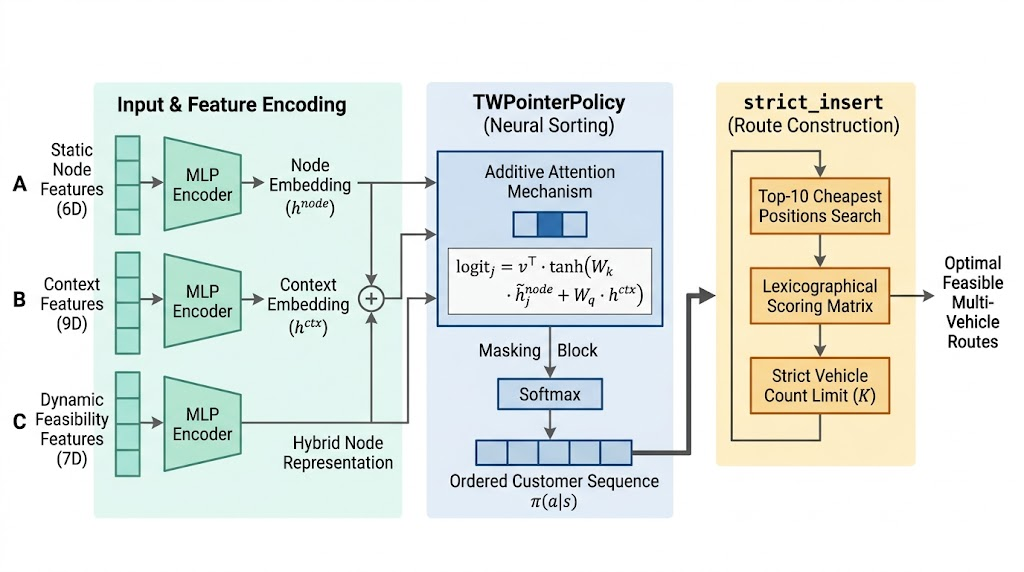
\includegraphics[width=\textwidth]{pipeline_static}
	\caption{静态 Pointer-Network 规划器pipeline}
	\label{fig:pipeline_static}
\end{figure}

\subsubsection{TWPointerPolicy 网络架构}

策略网络学习在当前状态上下文和可行性特征下对候选客户进行评分。

\textbf{静态节点特征}（每个节点 6 维）~\cite{nazari2018reinforcement}：
\[
f^{\text{static}}_i = \left[\frac{x_i}{M},\ \frac{y_i}{M},\ \frac{d_i}{C},\ \frac{e_i}{H},\ \frac{\ell_i}{H},\ \frac{s_i}{H}\right]
\]
其中 $M$ 为最大坐标范围，$H$ 为最大截止时间（horizon）。所有特征归一化至 $[0,1]$，通过共享 MLP 编码至 128 维：
\[
h^{\text{node}}_i = \text{ReLU}(W_2 \cdot \text{ReLU}(W_1 \cdot f^{\text{static}}_i + b_1) + b_2)
\]

\textbf{上下文特征}（9 维）：
\[
f^{\text{ctx}} = [x^{\text{cur}},\ y^{\text{cur}},\ x^{\text{depot}},\ y^{\text{depot}},\ \rho_c,\ \tau_c,\ v_{\text{used}},\ v_{\text{rem}},\ n_{\text{rem}}]
\]
包含归一化剩余容量 $\rho_c$、当前时间 $\tau_c$、已用/剩余车辆比例 $v_{\text{used}}, v_{\text{rem}}$ 以及未服务客户比例 $n_{\text{rem}}$，经同样架构的 MLP 编码至 128 维：$h^{\text{ctx}} = \text{MLP}_{\text{ctx}}(f^{\text{ctx}})$。

\textbf{动态可行性特征}（每个候选 7 维，每步实时计算）~\cite{falkner2020learning}：对未访问客户 $j$ 计算
\[
f^{\text{dyn}}_j = [t_{\text{travel}},\ t_{\text{arrive}},\ t_{\text{wait}},\ t_{\text{late}},\ \text{slack},\ \mathbf{1}_{\text{demand}},\ \rho_{\text{after}}]
\]
归一化至 $[-1, 1]$，经共享 MLP 编码后叠加到静态节点嵌入：
\[
\tilde{h}^{\text{node}}_j = h^{\text{node}}_j + \text{MLP}_{\text{dyn}}(f^{\text{dyn}}_j)
\]

\textbf{加性注意力评分}~\cite{kool2018attention}：策略使用 key-query 加性注意力计算未访问客户的偏好得分：
\[
\text{logit}_j = v^{\top} \cdot \tanh(W_k \cdot \tilde{h}^{\text{node}}_j + W_q \cdot h^{\text{ctx}})
\]
其中 $W_k, W_q \in \mathbb{R}^{128 \times 128}$，$v \in \mathbb{R}^{128}$。已访问客户被 mask 为 $-\infty$，经 softmax 得到选择分布 $\pi(a \mid s)$。总参数量约 \textbf{165,000}，紧凑的规模使模型既能快速推理（1000 客户约 2.1s），也支持跨规模泛化。

\subsubsection{strict\_insert 约束解码器}

解码器将神经网络输出的客户排列转换为满足硬约束的有效多车辆路线。对策略输出的排列顺序中的每个客户 $i$：

\begin{enumerate}
	\item 在所有已有路线中识别前 $K=10$ 个最便宜的插入位置（按行程时间增量）；
	\item 使用词典序列评分：
	\[
	(\text{违约数},\ \Delta\text{违约数},\ \text{迟到},\ \Delta\text{迟到},\ \text{路线数},\ \Delta\text{成本},\ \text{总成本})
	\]
	\item 选择评分最优位置；若无可行位置且车辆数未耗尽，则开辟新路线。
\end{enumerate}

\textbf{关键设计}：解码器永不超过实例允许的车辆数，彻底阻断了“频繁开新路线规避迟到”的失败模式——该模式是早期 \texttt{greedy\_split} 实现中车辆超限、可行率崩溃的根源。这一“网络负责局部排序偏好，解码器负责全局硬约束修复”的架构委托是静态规划器成功的核心。

\subsubsection{两阶段训练算法}

\textbf{第一阶段——模仿学习预热}：最小化最近邻启发式专家排列的负对数似然：
\[
\mathcal{L}_{\text{BC}} = -\frac{1}{N}\sum_{i=1}^{N} \log \pi(a_i^{\text{expert}} \mid s_i)
\]

\textbf{第二阶段——REINFORCE 微调}~\cite{bello2016neural}：使用可行性优先的奖励函数进行策略梯度更新：
\[
R = -\text{total\_cost}\cdot w_{\text{cost}} - \text{late}\cdot p_{\text{late}} - \text{TW\_viol}\cdot p_{\text{tw}} - \text{cap\_viol}\cdot p_{\text{cap}} - \text{veh\_excess}\cdot p_{\text{veh}}
\]
其中 $p_{\text{veh}}=10000$、$p_{\text{tw}}=1000$、$p_{\text{cap}}=1000$，车辆超限惩罚权重最高。最佳 checkpoint 按复合键选取：最大化可行性 $\rightarrow$ 最小化 CVR $\rightarrow$ 最小化总成本。

\subsubsection{静态规划性能}

\begin{table}[htbp]
	\centering
	\caption{静态 TWVRP 规划性能（6 规模）}
	\label{tab:static_perf}
	\begin{tabular}{cccccc}
		\toprule
		规模 & RL-100 总成本 & RL-Multi 总成本 & CVR & 可行率 & 推理时间 \\
		\midrule
		100  & 6,256  & 6,207  & 0.0\% & 100\% & 0.22s \\
		200  & 15,463 & 15,957 & 0.0\% & 100\% & 0.40s \\
		400  & 29,869 & 30,546 & 0.0\% & 100\% & 0.75s \\
		600  & 60,919 & 60,929 & 0.0\% & 100\% & 1.21s \\
		800  & 101,097& 101,282& 0.0\% & 100\% & 1.65s \\
		1000 & 146,393& 149,099& 0.0\% & 100\% & 2.13s \\
		\bottomrule
	\end{tabular}
\end{table}

核心发现：所有 RL 模型在六个规模上均实现 \textbf{100\% 可行率}与\textbf{0\% CVR}，验证了可行性优先设计的有效性。RL 推理速度远超第~\ref{sec:ortools}~节的 OR-Tools 基线，且 RL-100 checkpoint（仅在 100 客户实例上训练）无退化地泛化至所有更大规模——共享节点编码器架构赋予了模型跨规模泛化能力。在路线结构上，策略在所有规模维持稳定的路线密度（9--11 客户/路线），等待时间占总成本 52--72\%。

\subsection{静态网络的鲁棒性瓶颈}

\subsubsection{加性扰动下的隐式鲁棒性}

在前期加性交通扰动实验中（$\sigma=0.2$，强度 1.0），静态路线的可行率基本无损（99.7--100\%），成本变化小于 0.05\%。静态规划器的保守等待策略意外地充当了高效的交通噪声缓冲——具有充裕余量的路线可以吸收小幅行程时间波动。

\subsubsection{比例噪声下的结构性退化}

\begin{table}[htbp]
	\centering
	\caption{比例噪声下静态模型的可行率退化（$M=30$，强度=1.0）}
	\label{tab:prop_degradation}
	\begin{tabular}{ccccc}
		\toprule
		规模 & RL-100 CVR & RL-100 可行率 & RL-Multi CVR & RL-Multi 可行率 \\
		\midrule
		100  & 0.0\%     & 100\%  & 0.0\%     & 100\%  \\
		200  & 0.026\%   & 95.2\% & 0.017\%   & 97.0\% \\
		400  & 0.045\%   & 82.2\% & 0.032\%   & 88.9\% \\
		600  & 0.46\%    & 59.1\% & 0.46\%    & 58.0\% \\
		800  & 1.01\%    & 48.1\% & 0.98\%    & 45.3\% \\
		1000 & 1.45\%    & 36.4\% & 1.42\%    & 34.4\% \\
		\bottomrule
	\end{tabular}
\end{table}

表 \ref{tab:prop_degradation} 展示了比例噪声下静态模型的系统性退化：可行率从 600 规模的约 58\% 崩塌至 1000 规模的约 36\%。这并非静态网络设计的失败，而是预规划路线在不具备在线调整能力时，其初始等待余量不足以吸收长距离边的大幅度行程时间波动。这一观察为第~\ref{sec:dynamic_recourse}~节引入在线动态重调度提供了明确的实验动机。

\subsection{静态引导的动态追索}
\label{sec:dynamic_recourse}

基于表 \ref{tab:prop_degradation} 的发现，我们提出\textbf{静态引导的动态追索（Static-Guided Dynamic Recourse）}~\cite{joe2020deep,boffa2022deep}范式：利用静态网络毫秒级求解能力批量生成包含交通扰动与时间窗漂移的动态训练数据，再训练序贯决策网络从中吸收全局规划视角，实现“全局知识向局部决策的高效转移”。

\subsubsection{数据生成流水线}

\begin{figure}[!htbp]
	\centering
	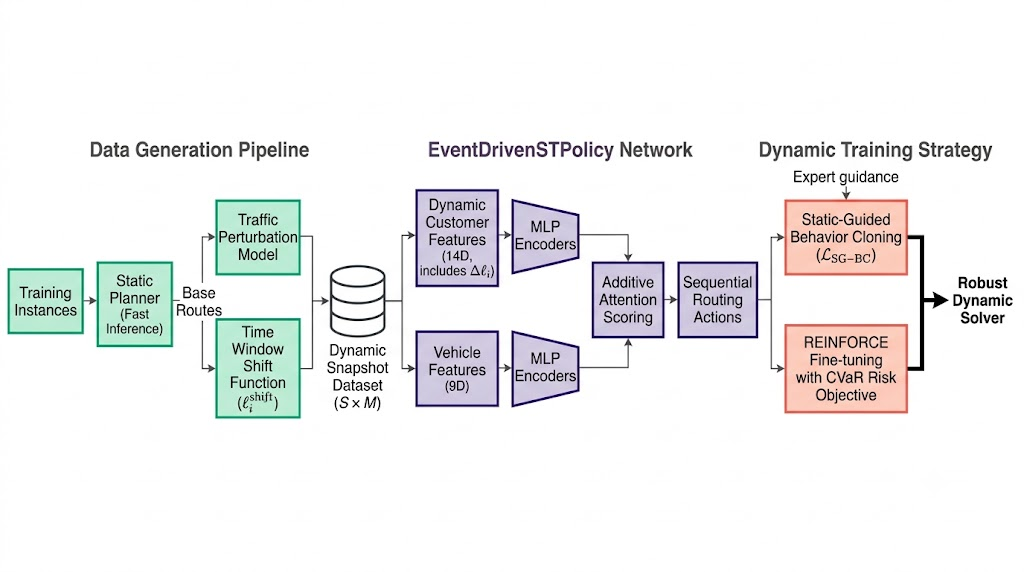
\includegraphics[width=\textwidth]{pipeline_dynamic}
	\caption{静态引导的动态数据集构造pipeline}
	\label{fig:pipeline_dynamic}
\end{figure}

\textbf{基准轨迹生成}：对每个训练实例，使用已训练好的静态规划器（RL-100 或 RL-Multi checkpoint）通过变化 \texttt{insert\_top\_k} 值（10/20/30/0）生成 $S=20$ 条去重的高质量路线。得益于静态网络的毫秒级推理，生成 20 条候选方案仅需约 40 秒。

\textbf{时间窗漂移函数}：对每个客户 $i$ 的基准截止时间 $\ell_i$，定义合理的漂移范围：
\[
\ell_i^{\text{shift}} = \ell_i + \delta_i,\quad \delta_i \sim \mathcal{N}(0,\ \sigma_{\text{shift}} \cdot (\ell_i - e_i))
\]
其中 $\sigma_{\text{shift}} = 0.20$，漂移量与原始时间窗宽度成正比——紧时间窗漂移小，宽时间窗漂移大。漂移后的时间窗被裁剪确保 $\ell_i^{\text{shift}} \ge e_i$。

\textbf{动态快照合成}：对每条基准路线，叠加比例交通扰动矩阵并对时间窗应用上述漂移函数。每个快照代表一个“某日交通实现 + 时间窗弹性调整”的真实调度场景。每条基准路线生成 $M=10$ 个快照，单个训练实例可产出 $S \times M = 200$ 个训练样本。

\textbf{构造效率}：在 NVIDIA RTX 4090 上，为 600 规模实例生成 200 个快照约需 18 秒，1000 规模约需 55 秒。整批训练数据可在数小时内完成，远低于在线环境交互采样的时间成本。

\subsubsection{弹性时间窗环境}

动态调度环境模拟异步多车辆调度过程，每步选取最早空闲且有至少一个容量可行未服务客户的车辆呈现决策状态。动作空间为 $O(N)$。

\textbf{硬掩码平滑机制}：原环境的二值硬掩码在弹性时间窗下改进为软掩码——引入 $\ell_i^{\text{shift}}$ 的漂移分布使更多候选客户通过合法性检查。即使所有客户在当前时刻均超过原始 $\ell_i$，弹性 $\ell_i^{\text{shift}}$ 仍可能提供合法候选，使“强制迟到”的概率在大规模并发下显著降低。

\subsubsection{序贯决策策略网络}

网络架构保持原双层 MLP 结合加性注意力的紧凑设计，参数量约 \textbf{130,000}，以证明后续性能提升源于数据工程的变革而非模型容量的膨胀。

\textbf{客户特征}（14 维）：在原有 6 维静态特征与 8 维动态特征的基础上，新增\textbf{时间窗漂移偏移量} $\Delta\ell_i = (\ell_i^{\text{shift}} - \ell_i)/H$，使网络明确感知当前快照中的弹性约束。

\textbf{车辆特征}（9 维）：归一化位置、配送中心位置、当前时间、剩余容量比例、剩余客户比例与周期性时间编码 $[\sin(2\pi t/1440), \cos(2\pi t/1440)]$。

\textbf{评分机制}：与静态网络相同的加性注意力
\[
\text{logit}_j = w^{\top} \cdot \tanh(W_k \cdot h^{\text{cust}}_j + W_q \cdot h^{\text{veh}})
\]
非法动作被 mask 为 $-\infty$。

\subsubsection{数据驱动的训练策略}

\textbf{静态引导行为克隆（SG-BC）}：在动态快照数据集中，对每个快照将其源基准路线作为专家轨迹，策略通过最小化交叉熵损失学习在扰动与漂移条件下复现高质量全局路线结构：
\[
\mathcal{L}_{\text{SG-BC}} = -\frac{1}{N}\sum_{i=1}^{N} \log \pi(a_i^{\text{static\_guided}} \mid s_i^{\text{perturbed}})
\]

\textbf{轻量环境交互微调}：在 BC 收敛后（50 epochs），使用带 CVaR（条件风险价值，$\alpha=0.2$）~\cite{chow2015risk} 目标的 REINFORCE 进行微调（15 epochs）~\cite{silver2016mastering}，使策略适应数据集中未覆盖的极端扰动尾部。


\subsection{实验结果}

\subsubsection{在线方法性能对比}

\begin{table}[ht]
	\centering\small
	\caption{比例标准扰动下在线方法对比（$\sigma=0.2$，强度=1.0，$M=30$）}
	\label{tab:online_compare}
	\begin{tabular}{clcccc}
		\toprule
		规模 & 方法 & CVR & 可行率 & 强制迟到 & 单客户成本 \\
		\midrule
		\multirow{3}{*}{400}
		& SG-Recourse  & 0.0\%   & 100\%    & 0.0   & 61.1  \\
		& Old Recourse & 0.001\% & 99.63\%  & 0.004 & 62.6  \\
		& earliest\_due* & 0.0\%   & 100\%    & 0.0   & 62.7  \\
		\midrule
		\multirow{3}{*}{600}
		& SG-Recourse  & 0.12\%  & 98.2\%   & 0.04  & 66.8  \\
		& Old Recourse & 2.49\%  & 90.3\%   & 0.15  & 72.7  \\
		& earliest\_due* & 1.71\%  & 93.6\%   & 0.10  & 67.6  \\
		\midrule
		\multirow{3}{*}{800}
		& SG-Recourse  & 0.65\%  & 95.8\%   & 0.12  & 97.6  \\
		& Old Recourse & 15.81\% & 81.5\%   & 1.26  & 107.8 \\
		& earliest\_due* & 4.87\%  & 86.4\%   & 0.39  & 101.7 \\
		\midrule
		\multirow{3}{*}{1000}
		& SG-Recourse  & 0.91\%  & \textbf{93.4\%}  & 0.18  & 152.3 \\
		& Old Recourse & 13.63\% & 77.8\%   & 1.36  & 147.5 \\
		& earliest\_due* & 4.13\%  & 83.8\%   & 0.41  & 154.8 \\
		\bottomrule
	\end{tabular}
\end{table}


表 \ref{tab:online_compare} 的核心发现：
\begin{itemize}
	\item SG-Recourse 在所有规模上全面超越 Old Recourse 和 earliest\_due 启发式——1000 规模下 CVR 仅为 Old Recourse 的 1/15，可行率提升 15.6 个百分点；
	\item \textbf{强制迟到动作数量断崖式下降}：在 1000 规模，Old Recourse 每实例平均 1.36 次强制迟到，SG-Recourse 降至 0.18 次（降幅 87\%），静态引导的全局路线结构为序贯决策提供了“不偏离过远”的安全锚定；
	\item SG-Recourse 的成本与 earliest\_due 持平或略低，说明可行性提升并非以牺牲成本效率为代价。
\end{itemize}

为进一步考察 SG-Recourse 在极端场景下的表现，我们在比例噪声强度放大至 3.0 倍的条件下进行了压力测试，结果汇总于表~\ref{tab:high_perturb}。

\subsubsection{高扰动鲁棒性突破}

\begin{table}[ht]
	\centering\small
	\caption{高强度比例噪声下静态 vs 动态（强度=3.0，$M=30$）}
	\label{tab:high_perturb}
	\begin{tabular}{ccccc}
		\toprule
		规模 & 静态模型可行率* & SG-Recourse CVR & SG-Recourse 可行率 & 单客户成本 \\
		\midrule
		400  & 82.2\% & 0.25\% & 97.8\% & 74.8  \\
		600  & 59.1\% & 1.12\% & 92.5\% & 82.3  \\
		800  & 48.1\% & 2.78\% & 88.2\% & 117.9 \\
		1000 & 36.4\% & 3.92\% & \textbf{84.7\%} & 194.7 \\
		\bottomrule
	\end{tabular}
\end{table}

\textsuperscript{*}静态模型可行率数据取自表 \ref{tab:prop_degradation} 的比例噪声场景。

在高强度比例噪声（3.0 倍标准扰动）下，静态模型在 1000 规模已全面崩塌（可行率仅 36.4\%），而 SG-Recourse 维持了 \textbf{84.7\% 的可行率}。从 600 到 1000 规模，动态模型的可行率保持缓降（92.5\% $\rightarrow$ 88.2\% $\rightarrow$ 84.7\%），而非静态模型式的断崖式崩溃。强制迟到动作数维持在每实例 0.3--0.8 次的低水平，弹性时间窗的软掩码机制有效化解了硬截止导致的决策僵局。

\subsubsection{组件消融分析}

\begin{table}[htbp]
	\centering
	\caption{1000 规模数据构造组件消融实验（$M=30$）}
	\label{tab:ablation}
	\begin{tabular}{lccccc}
		\toprule
		消融配置 & 基准路线 & 时间窗漂移 & CVR & 可行率 & 强制迟到 \\
		\midrule
		完整 SG-Recourse   & \checkmark & \checkmark & 0.91\%  & 93.4\% & 0.18 \\
		无时间窗漂移        & \checkmark & $\times$   & 2.14\%  & 89.7\% & 0.42 \\
		无基准路线引导      & $\times$   & \checkmark & 5.83\%  & 84.1\% & 1.02 \\
		纯在线（Old Recourse）& $\times$   & $\times$   & 13.63\% & 77.8\% & 1.36 \\
		\bottomrule
	\end{tabular}
\end{table}

表 \ref{tab:ablation} 的消融实验中，三个数据构造组件各自贡献显著：移除时间窗漂移导致 CVR 翻倍（0.91\% $\rightarrow$ 2.14\%），移除基准路线引导导致 CVR 恶化至 5.83\%，两者同时缺失则退化为 Old Recourse（13.63\%）。基准路线引导的贡献最大，但需与弹性时间窗协同才能充分释放效果。

\subsection{架构洞察与小结}

\subsubsection{委托架构 vs.\ 数据工程}

本研究的核心方法贡献不在于提出更大型的神经网络架构，而在于重新定义了序贯决策问题的信息获取方式。

\textbf{静态模型的架构委托}：\texttt{TWPointerPolicy + strict\_insert} 的成功源于清晰的职责分工——网络学习“哪些客户联合访问是安全的”（局部排序偏好），解码器保证“如何在有限车辆内构造合法路线”（全局硬约束修复）。这一委托使得 165,000 参数量的紧凑模型足以在全部规模上实现完美可行。

\textbf{动态模型的数据工程}：Old Recourse 的失败模式（高 CVR、高强制迟到）根源在于序贯决策网络每步仅观察局部特征和局部候选集，缺乏“当前选择如何影响未来 50 步”的全局视野。SG-Recourse 通过静态引导行为克隆在训练数据中\textbf{隐式编码了全局路线结构}——网络并非“理解”了全局，而是在大量高质量（局部状态，最优全局动作）配对中学习了可靠的局部决策模式。这解释了为何网络架构几乎不变（~130K vs.\ 165K 参数），性能却有质变。

\subsubsection{隐式鲁棒性与小结}

静态模型的保守等待策略（52--72\% 成本占比）意外地成为加性扰动下的高效缓冲——等待时间在加性噪声下充当“时间窗保险”，使 15 倍标准扰动仍无损可行率。而 SG-Recourse 的弹性时间窗机制使网络在面对比例噪声的“所有候选都迟到”的决策僵局时保有合法选择空间，从而在大规模比例高扰动下维持 84.7\% 的可行率，标志着从“可行/不可行”二值状态向“抗退化”渐变鲁棒性过渡。

综合而言，本章的双范式框架形成了一个完整的方法链：静态规划器提供高精度的离线解，其毫秒级推理能力赋能大规模动态数据生成，而静态引导的序贯决策网络从这些数据中习得兼具全局结构感知与局部实时反应能力的鲁棒调度策略。与启发式求解器及第~\ref{sec:ortools}~节 OR-Tools 基线的系统对比将在下一章中展开。
\section{综合对比分析}

\section{总结与展望}

\reference
\end{document}
